\pdfminorversion=4
\documentclass[aspectratio=169]{beamer}

\mode<presentation>
{
  \usetheme{default}
  \usecolortheme{default}
  \usefonttheme{default}
  \setbeamertemplate{navigation symbols}{}
  \setbeamertemplate{caption}[numbered]
  \setbeamertemplate{footline}[frame number]  % or "page number"
  \setbeamercolor{frametitle}{fg=white}
  \setbeamercolor{footline}{fg=black}
} 

\usepackage[english]{babel}
\usepackage[utf8x]{inputenc}
\usepackage{tikz}
\usepackage{courier}
\usepackage{array}
\usepackage{bold-extra}
\usepackage{minted}
\usepackage[thicklines]{cancel}
\usepackage{fancyvrb}
\usepackage{tabto}

\xdefinecolor{dianablue}{rgb}{0.18,0.24,0.31}
\xdefinecolor{darkblue}{rgb}{0.1,0.1,0.7}
\xdefinecolor{darkgreen}{rgb}{0,0.5,0}
\xdefinecolor{darkgrey}{rgb}{0.35,0.35,0.35}
\xdefinecolor{darkorange}{rgb}{0.8,0.5,0}
\xdefinecolor{darkred}{rgb}{0.7,0,0}
\definecolor{darkgreen}{rgb}{0,0.6,0}
\definecolor{mauve}{rgb}{0.58,0,0.82}

\title[01-intro]{Python/Numpy for High-Performance Numerical Processing}
\author{Jim Pivarski}
\institute{Princeton University}
\date{November 15, 2018}

\usetikzlibrary{shapes.callouts}

\begin{document}

\logo{\pgfputat{\pgfxy(0.11, 7.4)}{\pgfbox[right,base]{\tikz{\filldraw[fill=dianablue, draw=none] (0 cm, 0 cm) rectangle (50 cm, 1 cm);}\mbox{\hspace{-8 cm}
\includegraphics[height=1 cm]{princeton-logo-long.png}\mbox{\hspace{0.25 cm}}}}}}

\begin{frame}
  \titlepage
\end{frame}

\logo{\pgfputat{\pgfxy(0.11, 7.4)}{\pgfbox[right,base]{\tikz{\filldraw[fill=dianablue, draw=none] (0 cm, 0 cm) rectangle (50 cm, 1 cm);}\mbox{\hspace{-8 cm}
\includegraphics[height=1 cm]{princeton-logo.png}\mbox{\hspace{0.25 cm}}}}}}

% Uncomment these lines for an automatically generated outline.
%\begin{frame}{Outline}
%  \tableofcontents
%\end{frame}

% START START START START START START START START START START START START START

\begin{frame}{Why Python?}
\vspace{0.25 cm}
\begin{center}
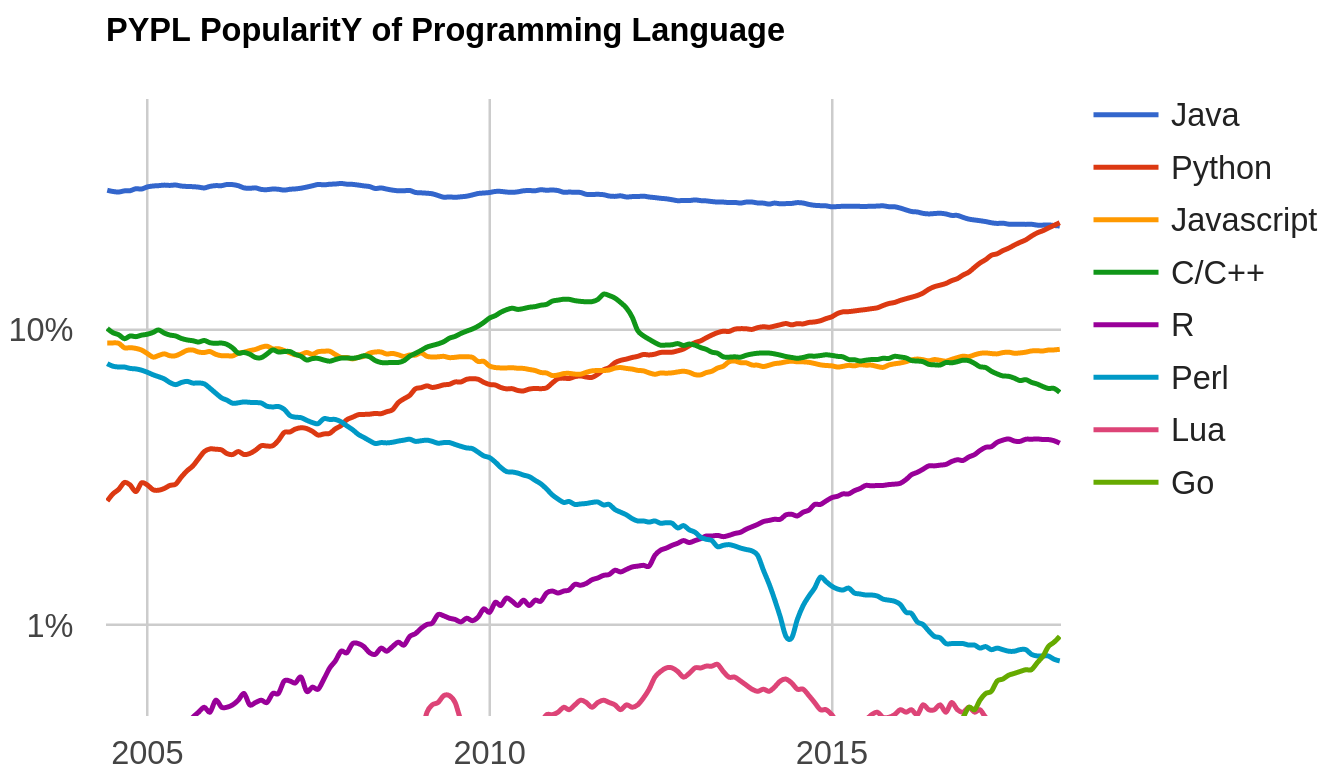
\includegraphics[width=0.8\linewidth]{pypl-popularity.png}

\textcolor{blue}{\scriptsize\url{http://pypl.github.io/PYPL.html}}
\end{center}
\end{frame}

\begin{frame}{Why Python in science?}
\vspace{0.5 cm}
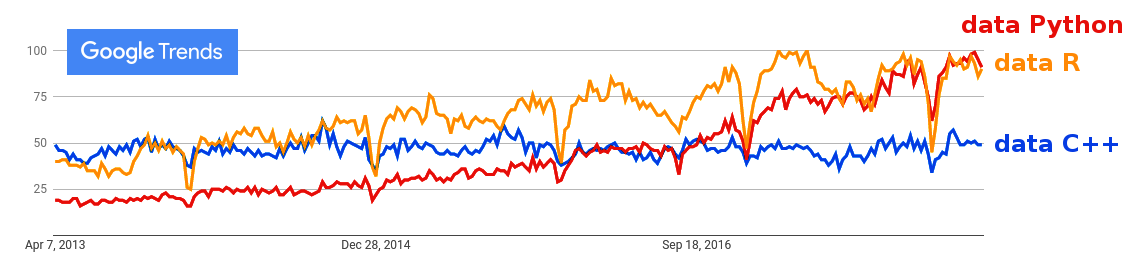
\includegraphics[width=\linewidth]{python-r-cpp-googletrends-data.png}

\vspace{1 cm}
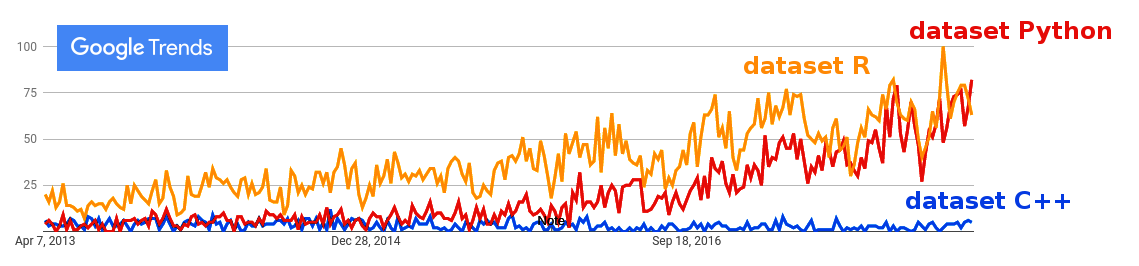
\includegraphics[width=\linewidth]{python-r-cpp-googletrends-dataset.png}
\end{frame}

\begin{frame}{Why Python in science?}
\vspace{0.5 cm}
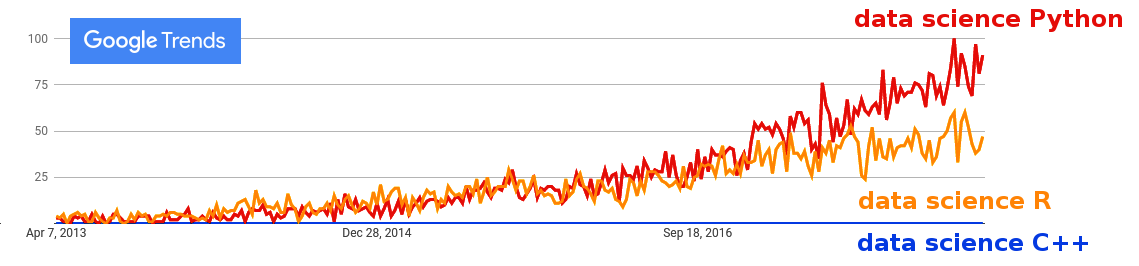
\includegraphics[width=\linewidth]{python-r-cpp-googletrends-datascience.png}

\vspace{1 cm}
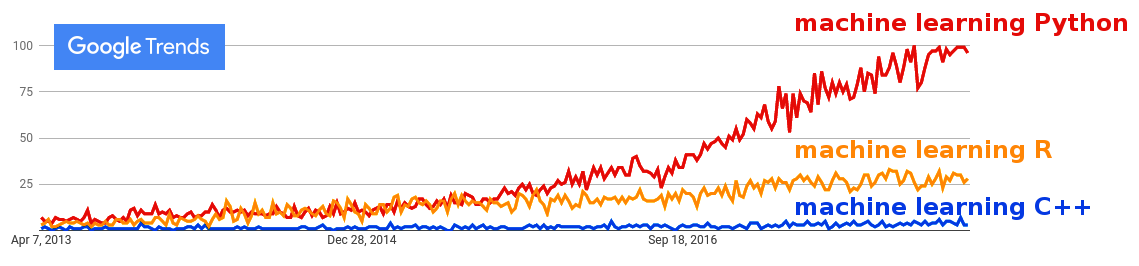
\includegraphics[width=\linewidth]{python-r-cpp-googletrends-machinelearning.png}
\end{frame}

\begin{frame}{Why Python in science?}
\vspace{0.5 cm}
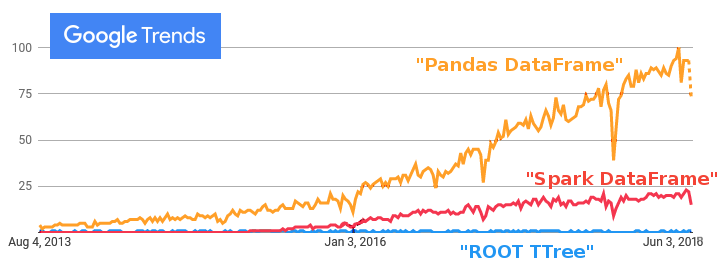
\includegraphics[width=\linewidth]{root-spark-pandas-google-trends.png}
\end{frame}

\begin{frame}{Why Python in science?}
\large
\vspace{0.4 cm}
All of the machine learning libraries I could find either have a Python interface or are primarily/exclusively Python.

\vspace{0.6 cm}
\mbox{ } 
\includegraphics[height=0.8 cm]{sklearn-logo.png}
\hfill 
\includegraphics[height=0.8 cm]{pytorch-logo.png}
\hfill 
\includegraphics[height=0.8 cm]{keras-logo.png}
\hfill 
\includegraphics[height=1 cm]{tensorflow-logo.png}
\hfill 
\includegraphics[height=0.8 cm]{caffe2-logo.png}
\hfill 
\includegraphics[height=0.8 cm]{gluon-logo.png} \mbox{ }

\vspace{0.15 cm}
\mbox{ } 
\includegraphics[height=0.8 cm]{chainer-logo.png}
\hfill 
\includegraphics[height=0.8 cm]{cntk-logo.png}
\hfill 
\includegraphics[height=0.8 cm]{lasagne-logo.png}
\hfill 
\includegraphics[height=0.8 cm]{onnx-logo.png}
\hfill 
\includegraphics[height=0.8 cm]{cesium-logo.png}
\hfill 
\includegraphics[height=0.8 cm]{xgboost-logo.png} \mbox{ }
\end{frame}

\begin{frame}{Why Python in science?}
\vspace{0.25 cm}
\begin{center}
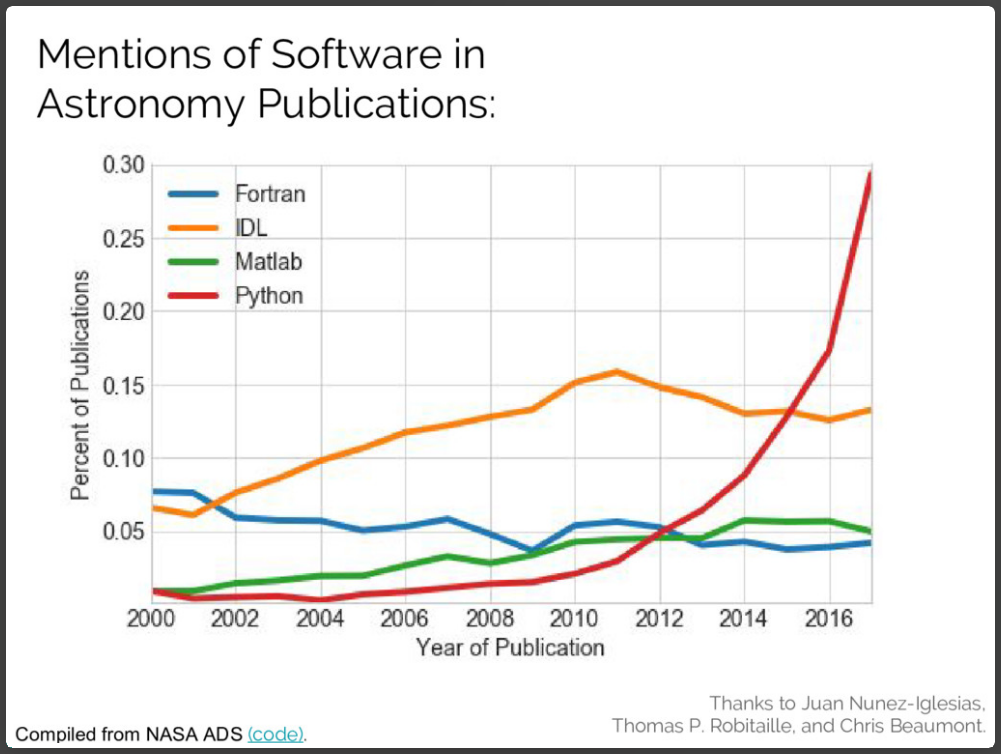
\includegraphics[width=0.7\linewidth]{mentions-of-programming-languages.png}
\end{center}
\end{frame}

\begin{frame}{Why Python in science?}
\vspace{0.3 cm}
\begin{columns}[b]
\column{0.59\linewidth}
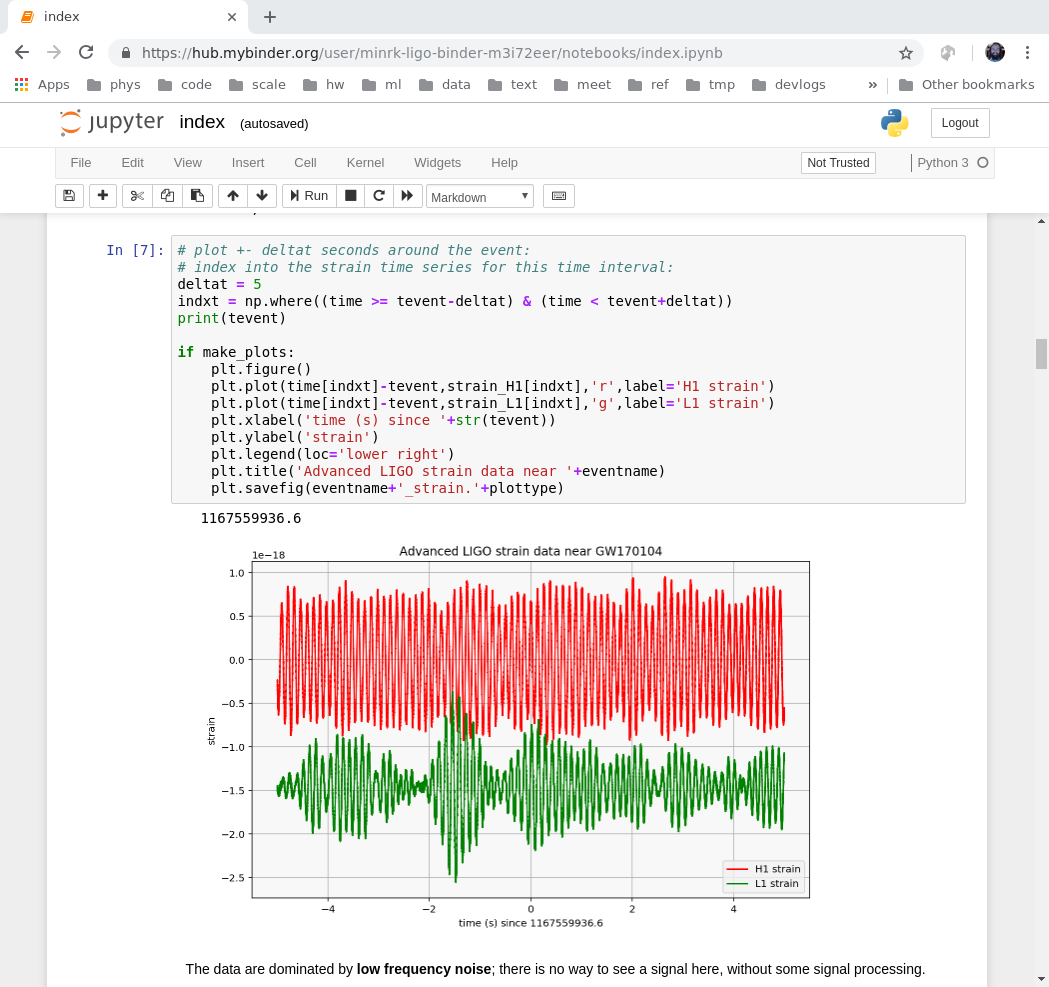
\includegraphics[width=\linewidth]{lsst-notebook.png}
\end{columns}
\end{frame}

\begin{frame}{Stealing from Jake VanderPlas's {\it Unexpected Effectiveness} talk}
\vspace{0.25 cm}
\begin{columns}[b]
\column{0.75\linewidth}
\only<1>{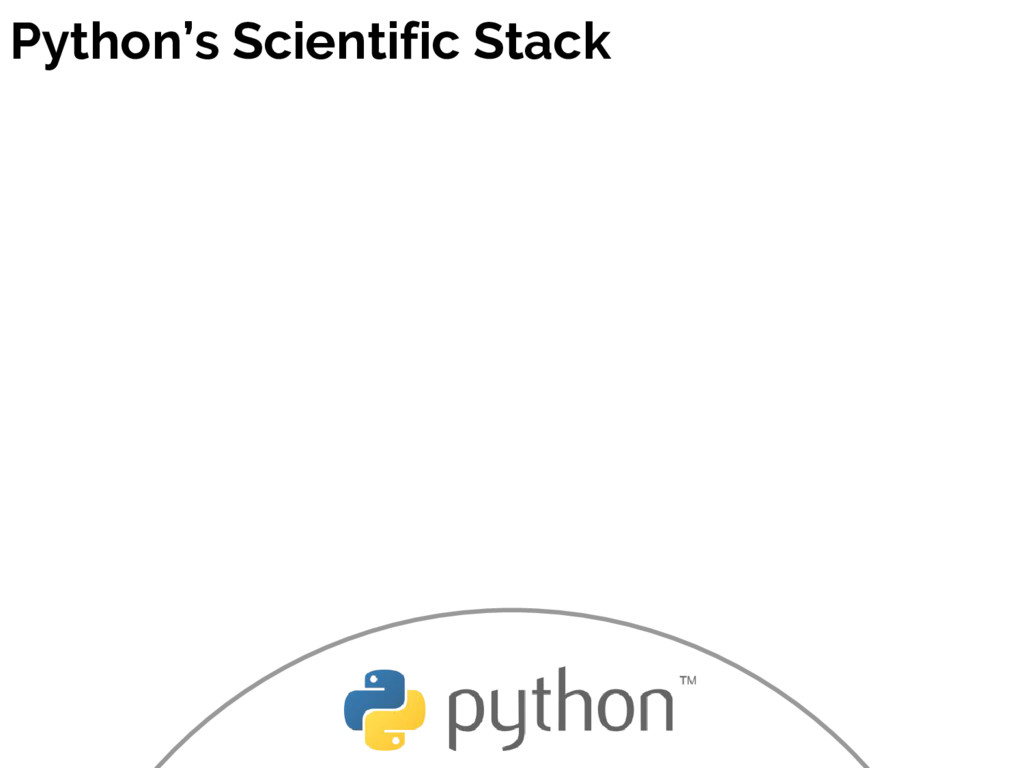
\includegraphics[height=7.8 cm]{shells-1.png}}
\only<2>{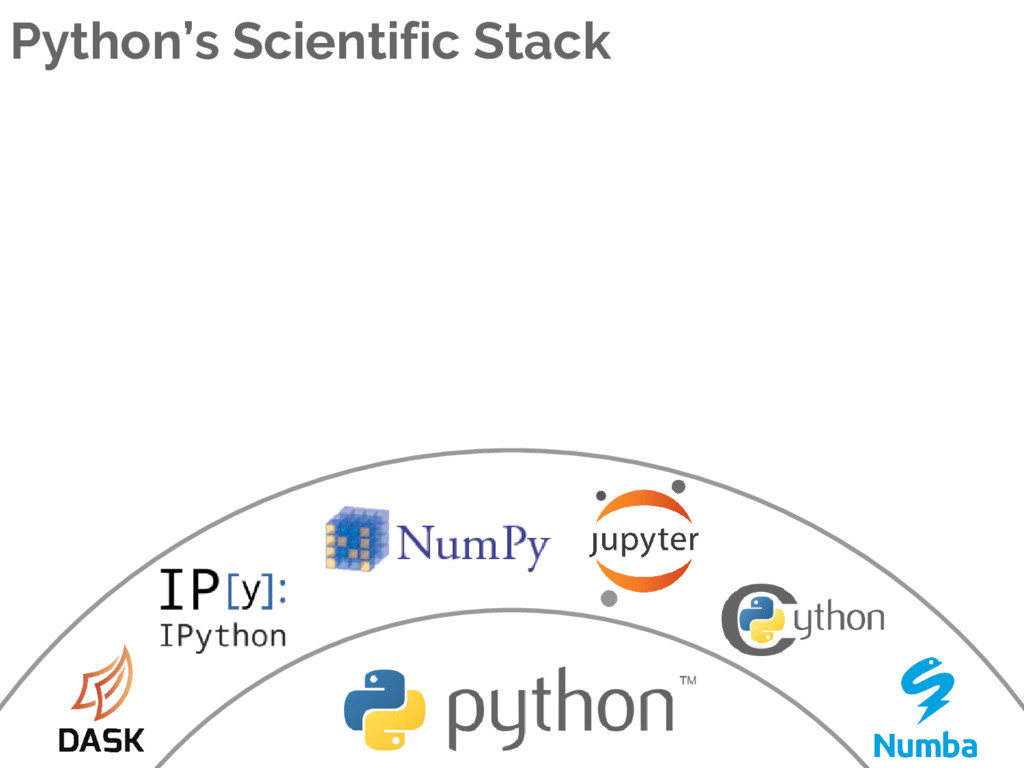
\includegraphics[height=7.8 cm]{shells-2.png}}
\only<3>{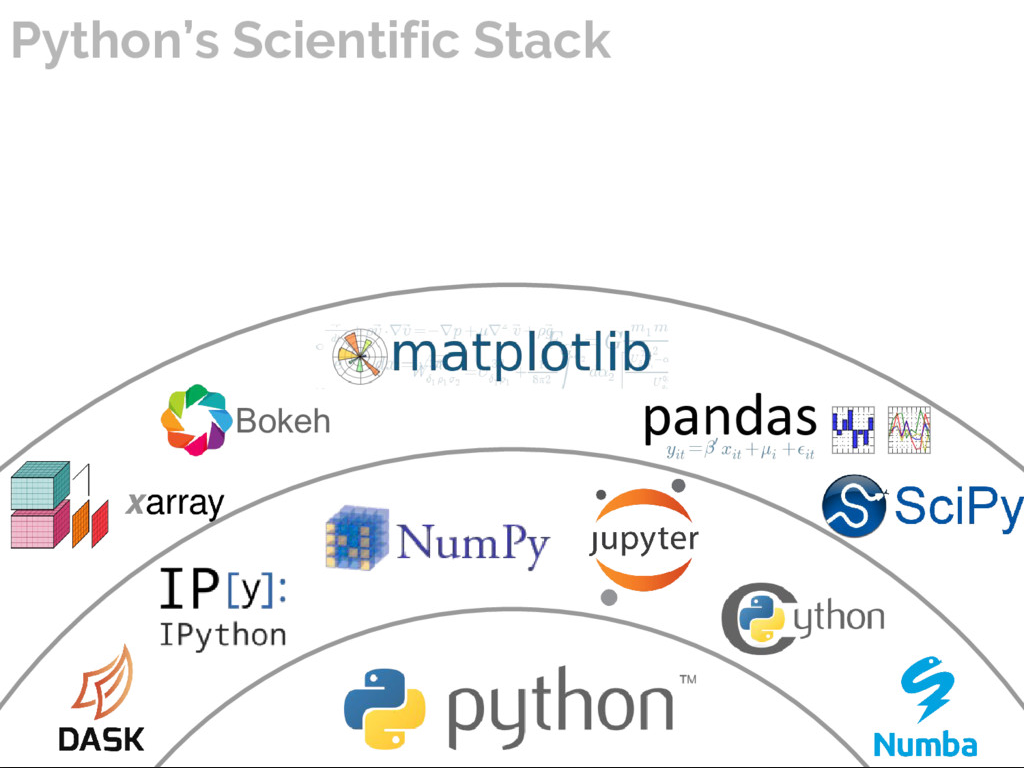
\includegraphics[height=7.8 cm]{shells-3.png}}
\only<4>{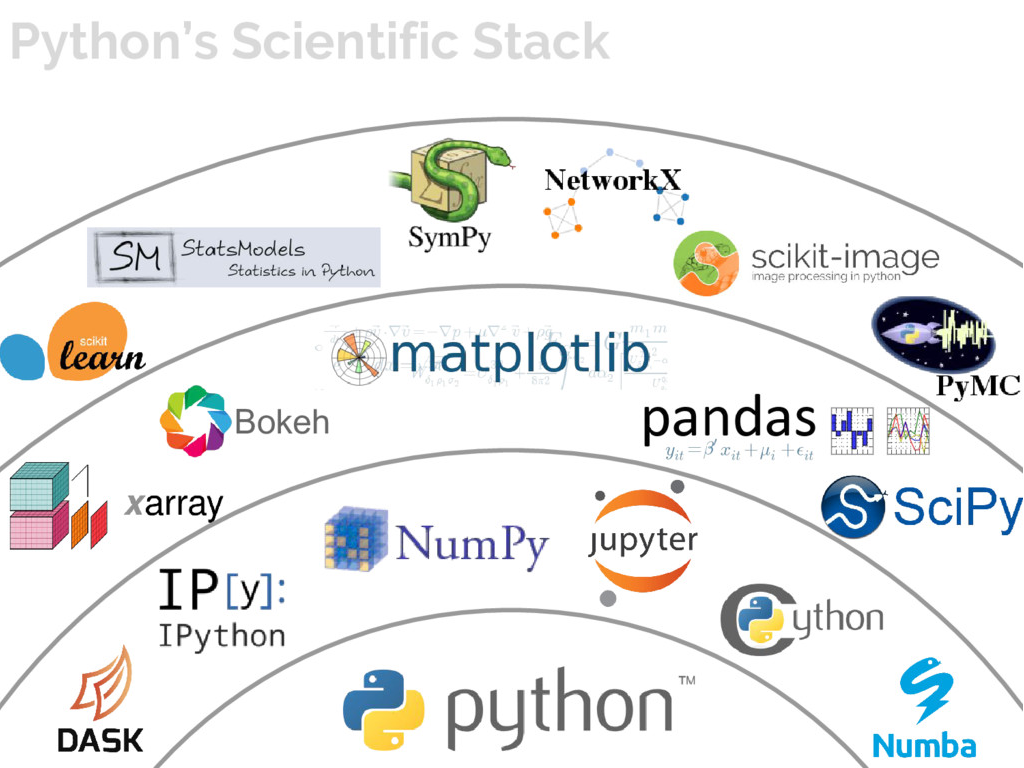
\includegraphics[height=7.8 cm]{shells-4.png}}
\only<5-6>{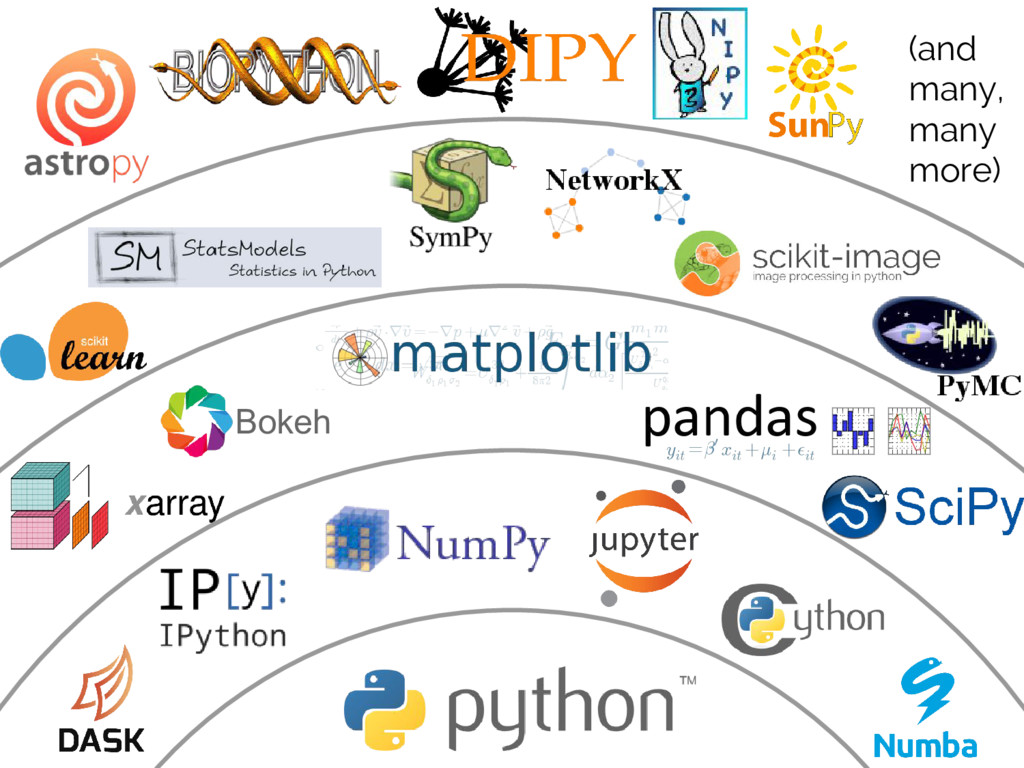
\includegraphics[height=7.8 cm]{shells-5.png}\vspace{0.5 cm}}

\column{0.25\linewidth}

\includegraphics[width=\linewidth]{unreasonable-effectiveness.png}

\vspace{0.5 cm}
\uncover<6>{If you're used to writing your own code, searching for tools is eye-opening: you learn what's unique about what you do and what isn't.}

\vspace{-7\baselineskip}
\vspace{4.8 cm}
\end{columns}
\end{frame}

\begin{frame}{Stealing again from Jake VanderPlas}
\vspace{0.27 cm}
\begin{columns}
\column{0.74\linewidth}
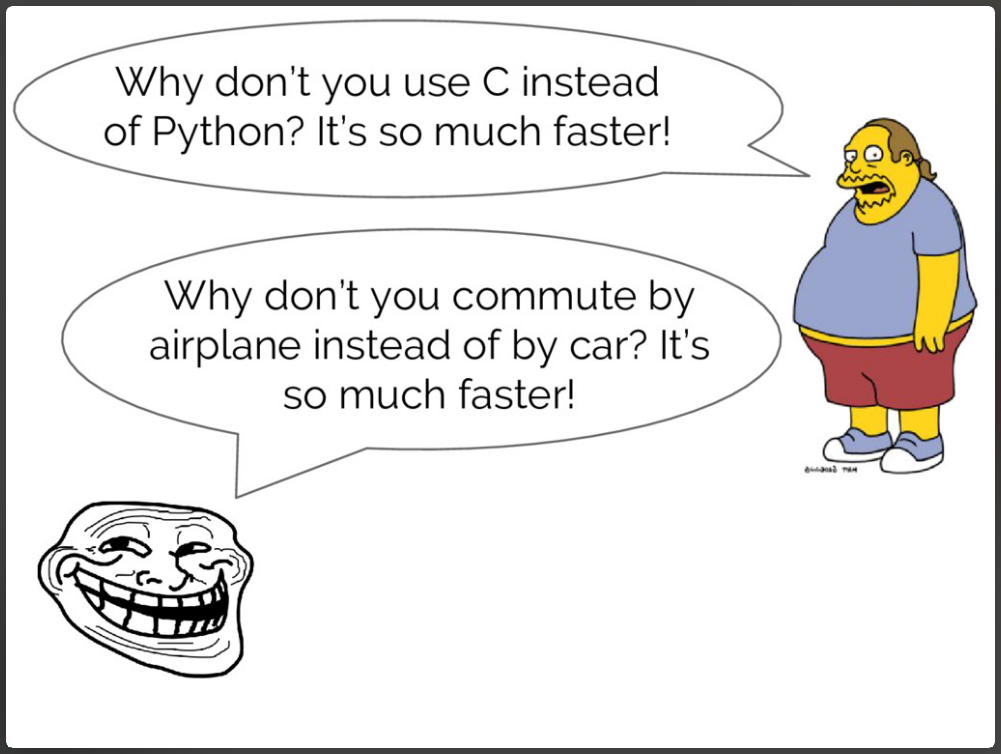
\includegraphics[width=\linewidth]{commute-by-plane.png}
\end{columns}
\end{frame}

\begin{frame}{Why not indeed?}
\large
\begin{center}
In science, we often have to scale up analyses to large datasets.

\vspace{1 cm}
\uncover<2->{10\% faster doesn't mean much, but the difference between \\ ``five minutes'' and ``overnight'' is life-changing.}

\vspace{1 cm}
\uncover<3->{That's the scale we're talking about between C and Python.}

\vspace{1 cm}
\uncover<4->{But we also need the interactivity of a dynamic language to {\it develop} the analysis. (``If we knew what we were doing, it wouldn't be called research.'')}
\end{center}
\end{frame}

\begin{frame}{Metaphor time!}
\Large
\vspace{0.25 cm}
\begin{center}
\textcolor{darkblue}{\underline{Drive to the airport by car, then take a plane.}}
\end{center}

\vspace{0.5 cm}
\begin{columns}
\column{0.4\linewidth}
\begin{center}
Small-scale {\it project organization} in Python, ignoring performance entirely.
\end{center}

\column{0.4\linewidth}
\begin{center}
Run over {\it big data} in compiled code, tuning performance until it no longer matters.
\end{center}

\end{columns}
\end{frame}

\begin{frame}{Python is a good glue language: my thesis workflow in 2006}
\vspace{0.5 cm}
\begin{columns}
\column{1.1\linewidth}
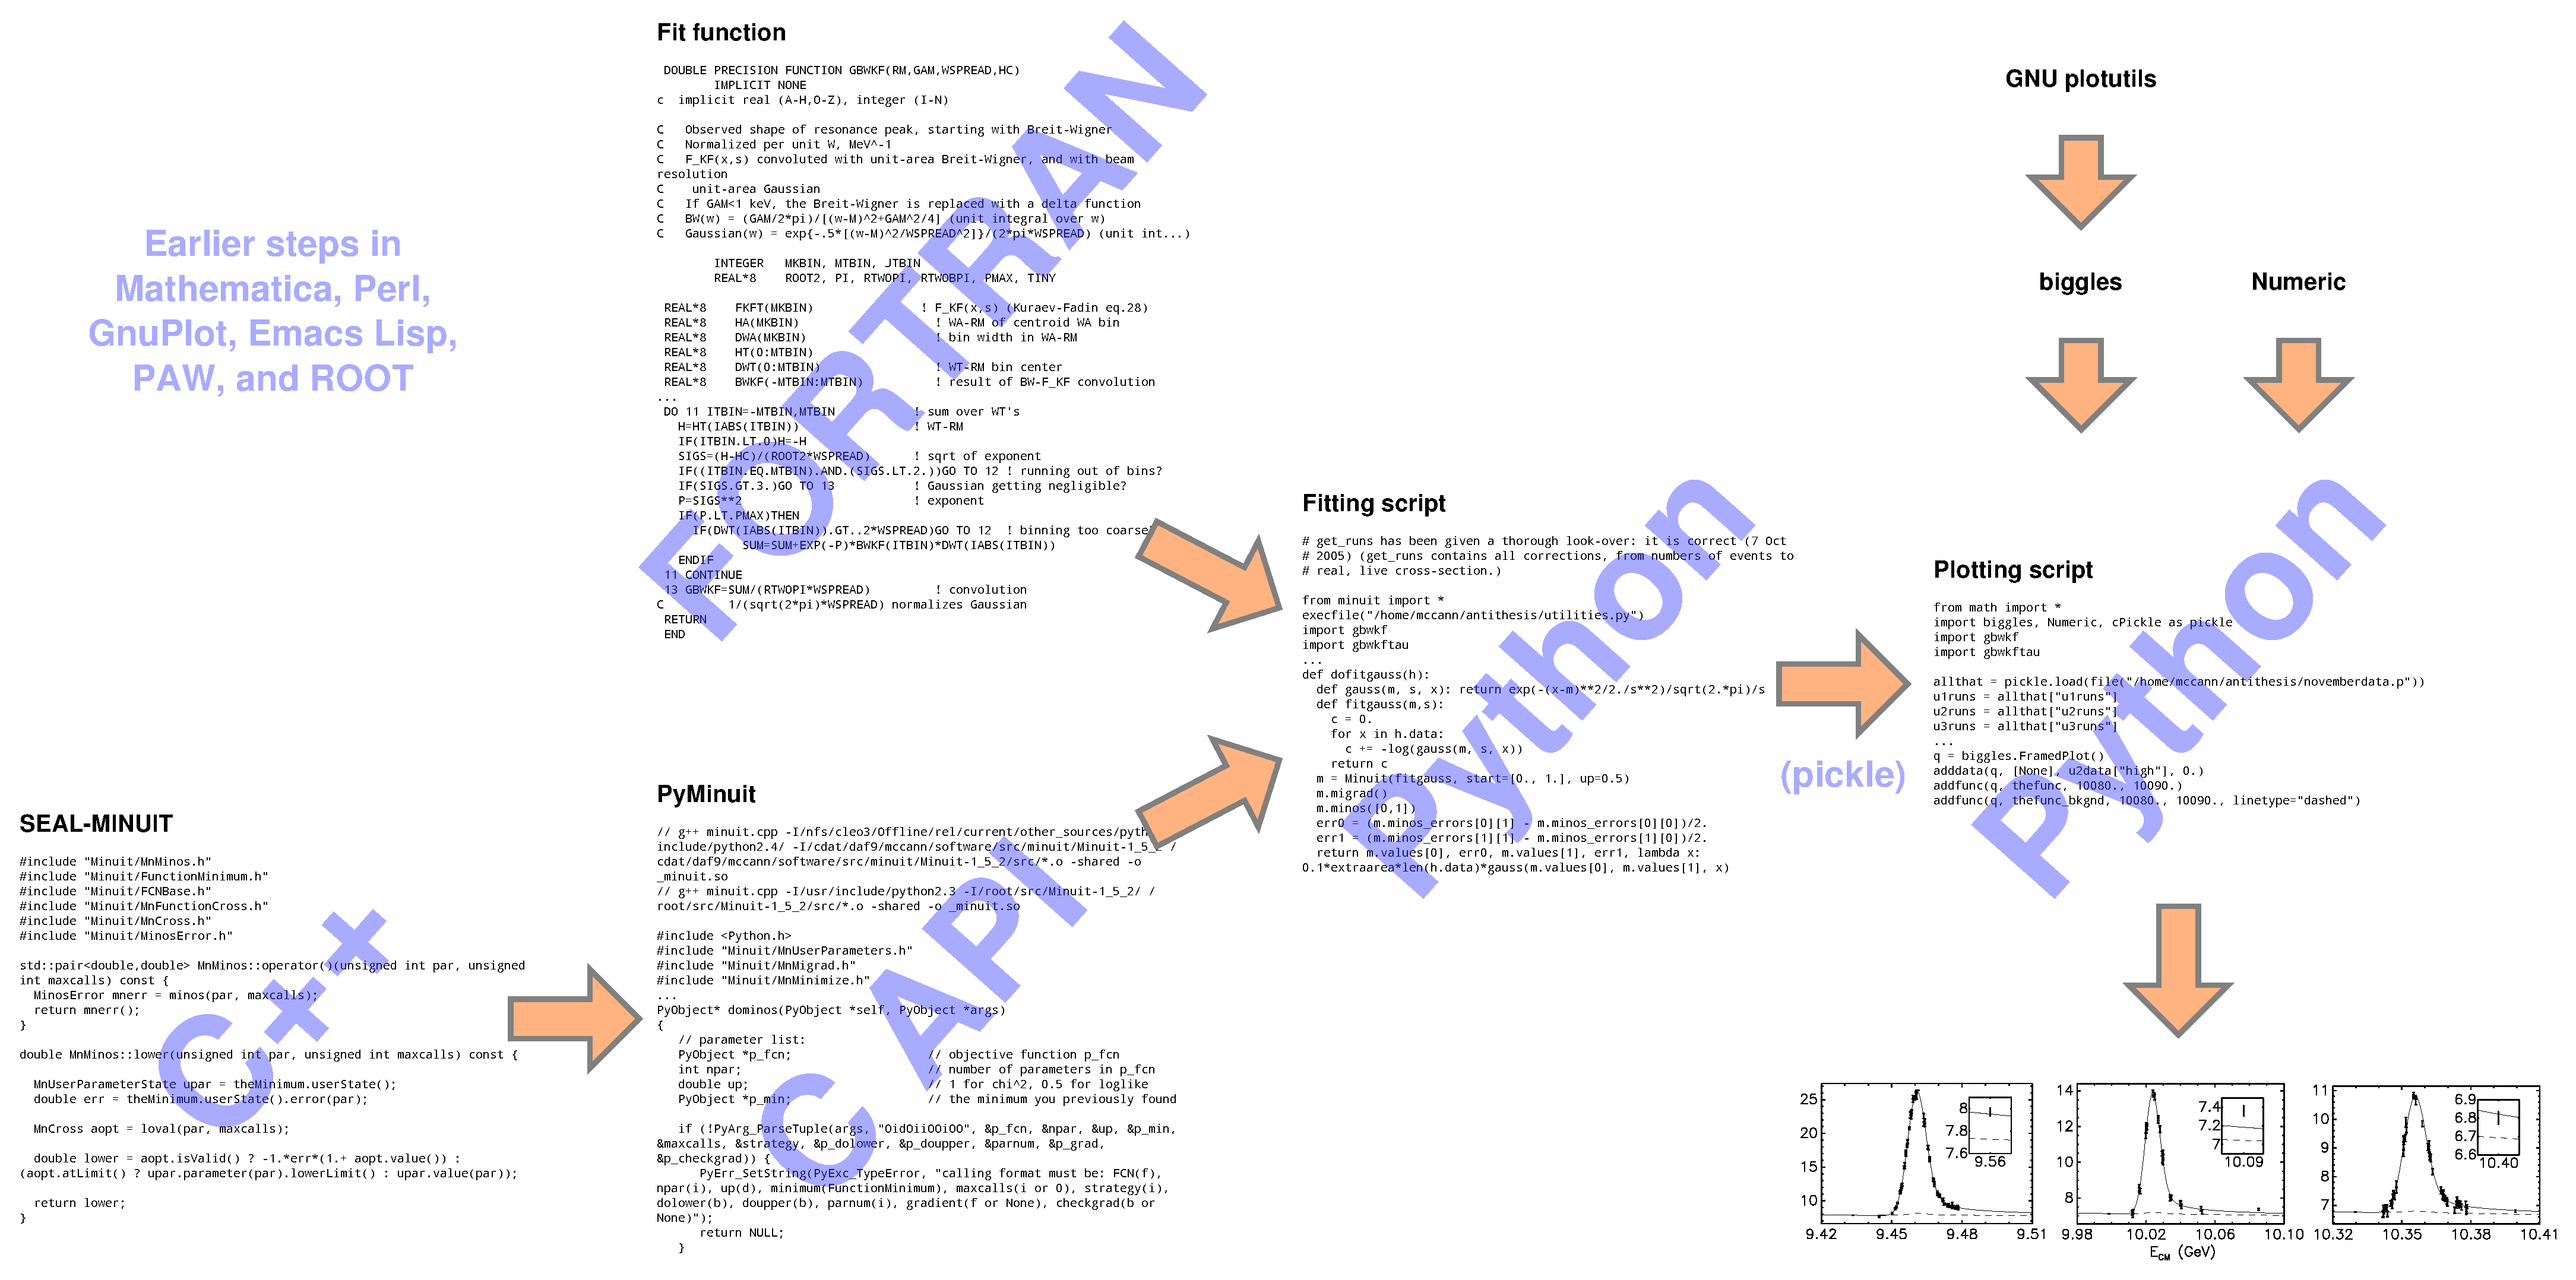
\includegraphics[width=\linewidth]{thesis-code-flow.pdf}
\end{columns}
\end{frame}

\begin{frame}{Which got me involved in open source (PyMinuit is now ``iminuit'')}
\vspace{0.5 cm}
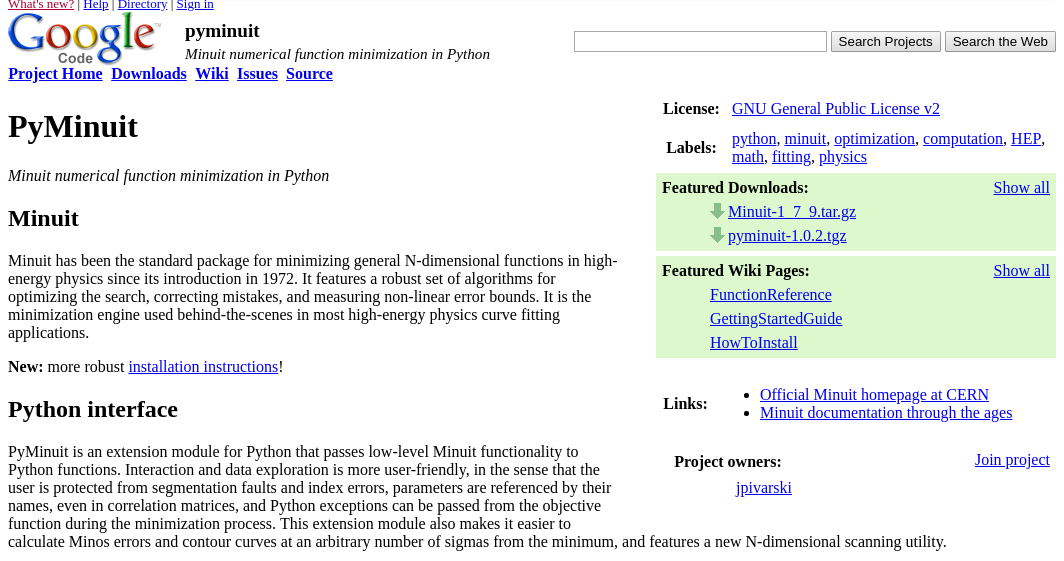
\includegraphics[width=\linewidth]{pyminuit.png}
\end{frame}

\begin{frame}{The key to ecosystem development was a common array library}
\large
\vspace{0.1 cm}

\renewcommand{\arraystretch}{1.15}
\mbox{\hspace{-0.5 cm}\begin{tabular}{c p{0.95\linewidth}}
1994 & \textcolor{darkorange}{\bf Python} 1.0 released. \\
1995 & First array package: \textcolor{darkorange}{\bf Numeric} \textcolor{gray}{(a.k.a.\ Numerical, Numerical Python, NumPy).} \\
2001 & Diverse scientific codebases merged into \textcolor{darkorange}{\bf SciPy}. \\
2003 & \textcolor{darkorange}{\bf Matplotlib} \\
2003 & Numeric was limited; \textcolor{darkorange}{\bf numarray} appeared as a competitor with more \mbox{features} \textcolor{gray}{(memory-mapped files, alignment, record arrays)}. \\
2005 & Two packages were incompatible; could not integrate numarray-based code into SciPy. Travis Oliphant merged the codebases as \textcolor{darkorange}{\bf Numpy}. \\
2008 & \textcolor{darkorange}{\bf Pandas} \\
2010 & \textcolor{darkorange}{\bf Scikit-Learn} \\
2011 & \textcolor{darkorange}{\bf AstroPy} \\
2012 & \textcolor{darkorange}{\bf Anaconda} \\
2014 & \textcolor{darkorange}{\bf Jupyter} \\
2015 & \textcolor{darkorange}{\bf Keras} \\
\end{tabular}}

\begin{uncoverenv}<2->
\vspace{-3 cm}
\hfill \fbox{\begin{minipage}{7 cm}
\vspace{0.2 cm}
\begin{center}
\begin{minipage}{6.25 cm}
The scientific Python ecosystem could have failed before it started if the Numeric/numarray split hadn't been resolved!
\end{minipage}
\vspace{0.2 cm}
\end{center}
\end{minipage}}
\end{uncoverenv}
\end{frame}

\begin{frame}[fragile]{Numpy is high-level, array-at-a-time math}
\vspace{0.5 cm}
\hfill 
\includegraphics[height=1.5 cm]{numpy-logo.png}

\scriptsize
\vspace{-1.6 cm}
\begin{minted}{python}
>>> import numpy
>>> a = numpy.arange(12)
>>> a
array([ 0,  1,  2,  3,  4,  5,  6,  7,  8,  9, 10, 11])
>>> a.shape = (3, 4)
>>> a
array([[ 0,  1,  2,  3],
       [ 4,  5,  6,  7],
       [ 8,  9, 10, 11]])
>>> a.sum(axis=0)
array([12, 15, 18, 21])
>>> a.min(axis=1)
array([0, 4, 8])
>>> a**2
array([[  0,   1,   4,   9],
       [ 16,  25,  36,  49],
       [ 64,  81, 100, 121]])
>>> numpy.sqrt(a)
array([[0.        , 1.        , 1.41421356, 1.73205081],
       [2.        , 2.23606798, 2.44948974, 2.64575131],
       [2.82842712, 3.        , 3.16227766, 3.31662479]])
\end{minted}
\end{frame}

\begin{frame}[fragile]{The Numpythonic mindset}
\large
\vspace{0.5 cm}
Although you can write Python {\tt\normalsize for} loops over Numpy arrays, you don't reap the benefit unless you express your calculation in Numpy universal functions (ufuncs).

\vspace{\baselineskip}
\begin{columns}[t]
\column{0.45\linewidth}
\vspace{-\baselineskip}
\scriptsize
\begin{minted}{python}
pz = numpy.empty(len(pt))
for i in range(len(pt)):
    pz[i] = pt[i]*numpy.sinh(eta[i])
\end{minted}

\vspace{0.5 cm}
$\mathcal{O}(N)$ Python bytecode instructions, type-checks, interpreter locks.

\column{0.45\linewidth}
\mbox{\hspace{-0.85 cm}\textcolor{darkblue}{vs}}
\vspace{-\baselineskip}
\scriptsize
\begin{minted}{python}
pz = pt * numpy.sinh(eta)
\end{minted}
\vspace{2\baselineskip}

\vspace{0.5 cm}
$\mathcal{O}(1)$ Python bytecode instructions, type-checks, interpreter locks.

\vspace{0.1 cm}
$\mathcal{O}(N)$ statically typed, probably vectorized native bytecode operations on contiguous memory.
\end{columns}

\large
\vspace{0.75 cm}
\uncover<2->{\textcolor{darkblue}{In other words, a \underline{S}ingle (Python) \underline{I}nstruction on \underline{M}ultiple \underline{D}ata.}}

\vspace{0.1 cm}
\uncover<2->{\textcolor{darkblue}{Conceptually similar to SIMD, the program flow of GPUs.}}
\end{frame}

\begin{frame}{This is not new}
\Large
\vspace{0.5 cm}
\textcolor{darkorange}{\bf APL}, ``A Programming Language'' introduced the idea of single commands having sweeping effects across large arrays.

\begin{center}
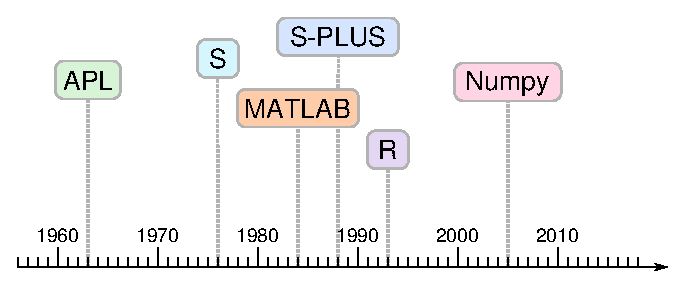
\includegraphics[width=0.75\linewidth]{apl-timeline.pdf}
\end{center}

\normalsize
\textcolor{gray}{All members of the APL family are intended for interactive data analysis.}

\textcolor{gray}{Numpy, however, is a library in a general-purpose language, not a language in itself.}
\end{frame}

\begin{frame}{APL}
\Large
\vspace{0.5 cm}
\hfill \mbox{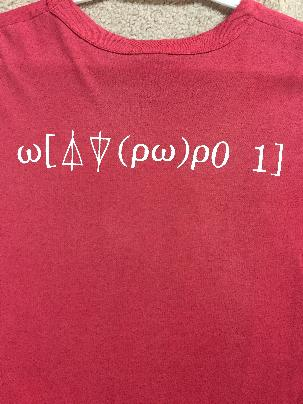
\includegraphics[height=3 cm]{tshirt.jpg}\hspace{-0.25 cm}}

\vspace{-2.75 cm}
APL pioneered conciseness;

discovered the mistake of being too concise.

\large
\vspace{1.25 cm}
Conway's Game of Life was one line of code:

\vspace{-0.3 cm}
\[ \mbox{\tt life} \leftarrow \{\uparrow 1\quad\omega \vee.\wedge 3\quad 4=+/,^{^-} 1\quad0\quad1\circ.\Theta^{^-} 1\quad0\quad1\circ.\Phi\subset\omega\} \]

\vspace{0.5 cm}
``Map'' was implicit, ``reduce'' was a slash, functions were symbols. For example:

\begin{center}
\renewcommand{\arraystretch}{1.2}
\begin{tabular}{c c c}
APL & \mbox{\hspace{0.5 cm}} & Numpy \\\hline
$\displaystyle \mbox{\tt m} \leftarrow +/(3+\iota 4)$ & & {\tt\normalsize m = (numpy.arange(4) + 3).sum()}
\end{tabular}
\end{center}
\end{frame}

\begin{frame}{Numpythonic mindset: GPU and vectorization}
\Large
\vspace{0.5 cm}
\begin{center}
As an array abstraction, Numpy presents a high-level way \\ for users to think about vectorization.

\vspace{1 cm}
Vectorization is key to using GPUs and modern CPUs efficiently.
\end{center}
\end{frame}

\begin{frame}{Numpythonic mindset: GPU and vectorization}
\vspace{0.35 cm}
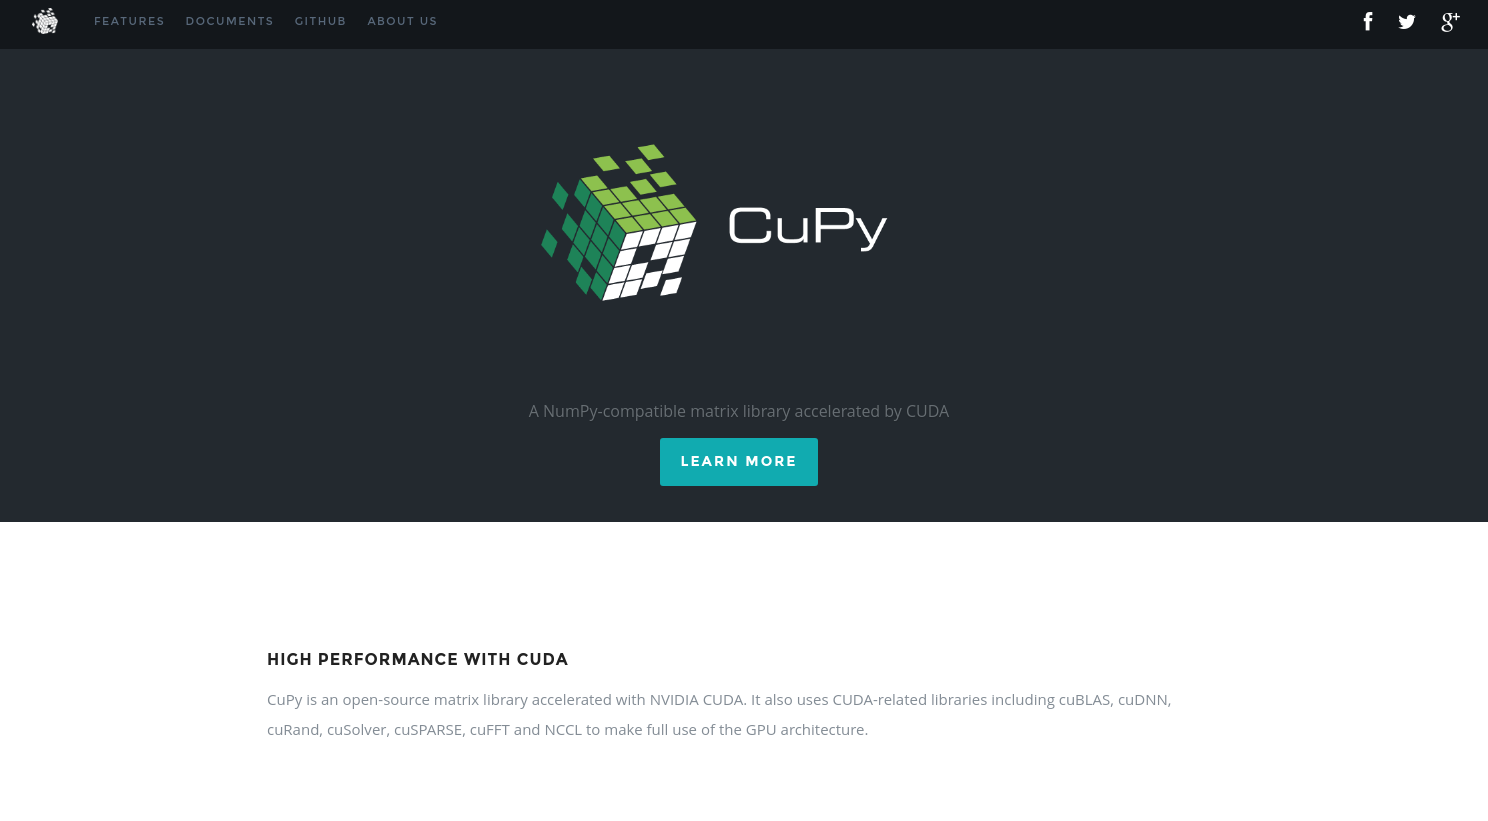
\includegraphics[width=\linewidth]{cupy.png}
\end{frame}

\begin{frame}{Numpythonic mindset: GPU and vectorization}
\vspace{0.35 cm}
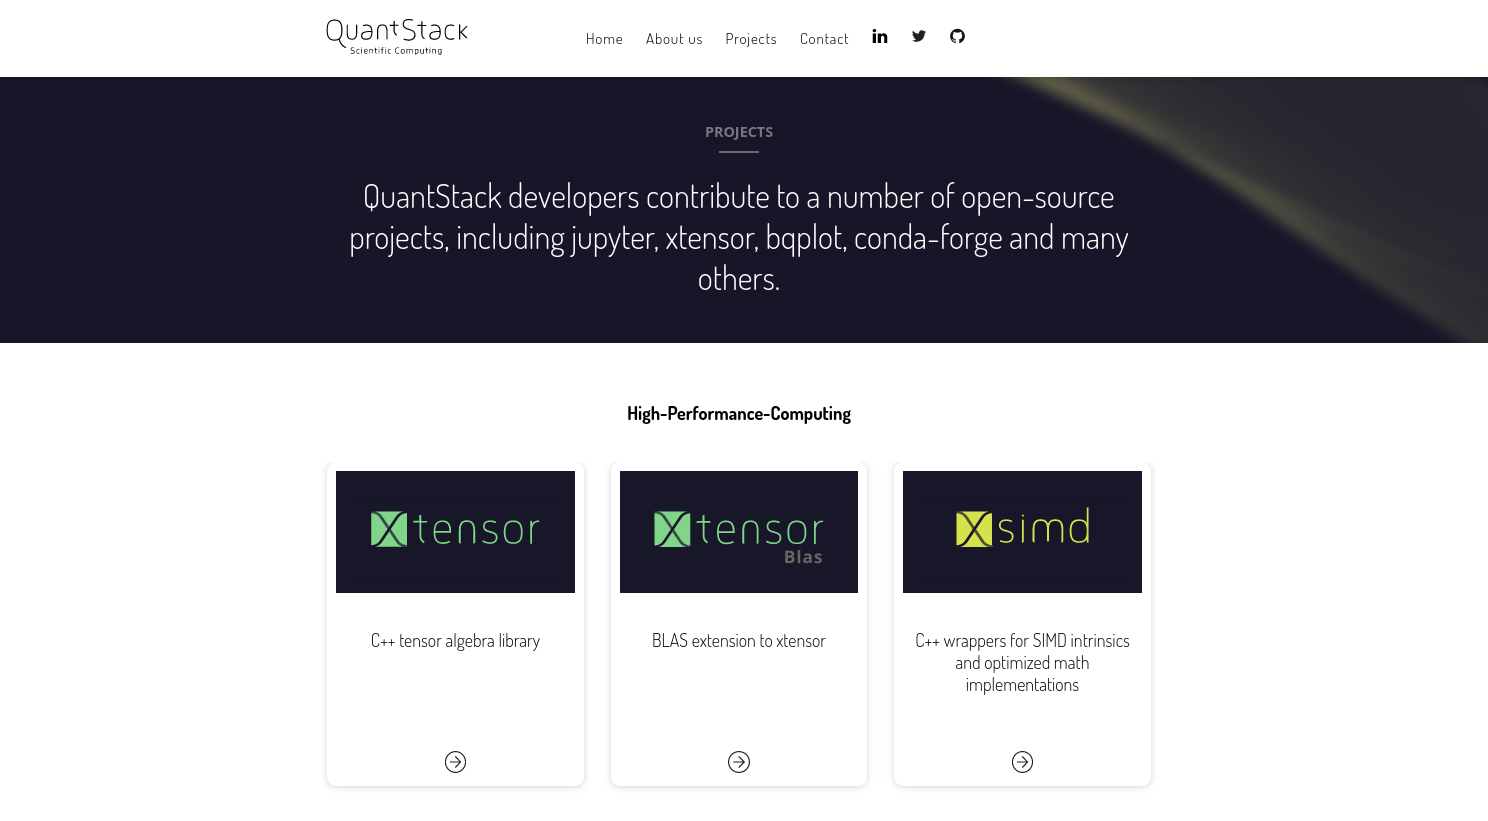
\includegraphics[width=\linewidth]{quantstack.png}
\end{frame}

\begin{frame}{Plan for the day}
\large
\begin{columns}
\column{0.68\linewidth}
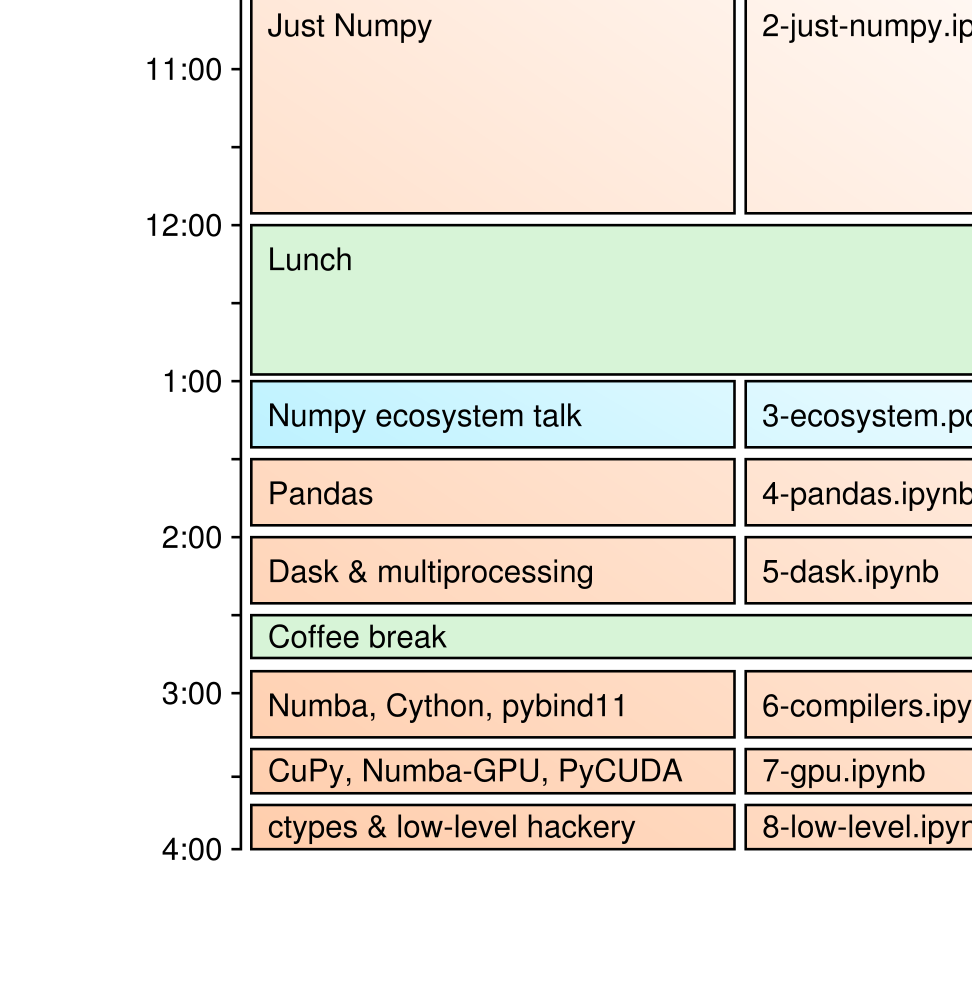
\includegraphics[width=\linewidth]{../img/plan-for-the-day.png}

\column{0.3\linewidth}
Skills-based Numpy tutorial with exercises in the morning: how to think in SIMD.

\vspace{1 cm}
Overview of libraries in the afternoon: where to look for solutions to your problems.
\end{columns}
\end{frame}

\end{document}
